% !TEX root = ../main.tex

% 附录A
\chapter{带章节的附录}[Full Appendix]

完整的附录内容,包含章节,公式,图表等。

\section{附录节的内容}[Section in Appendix]

这是附录的节的内容。

附录中\figref{fig:appA}:
\begin{figure}[htbp]
\centering
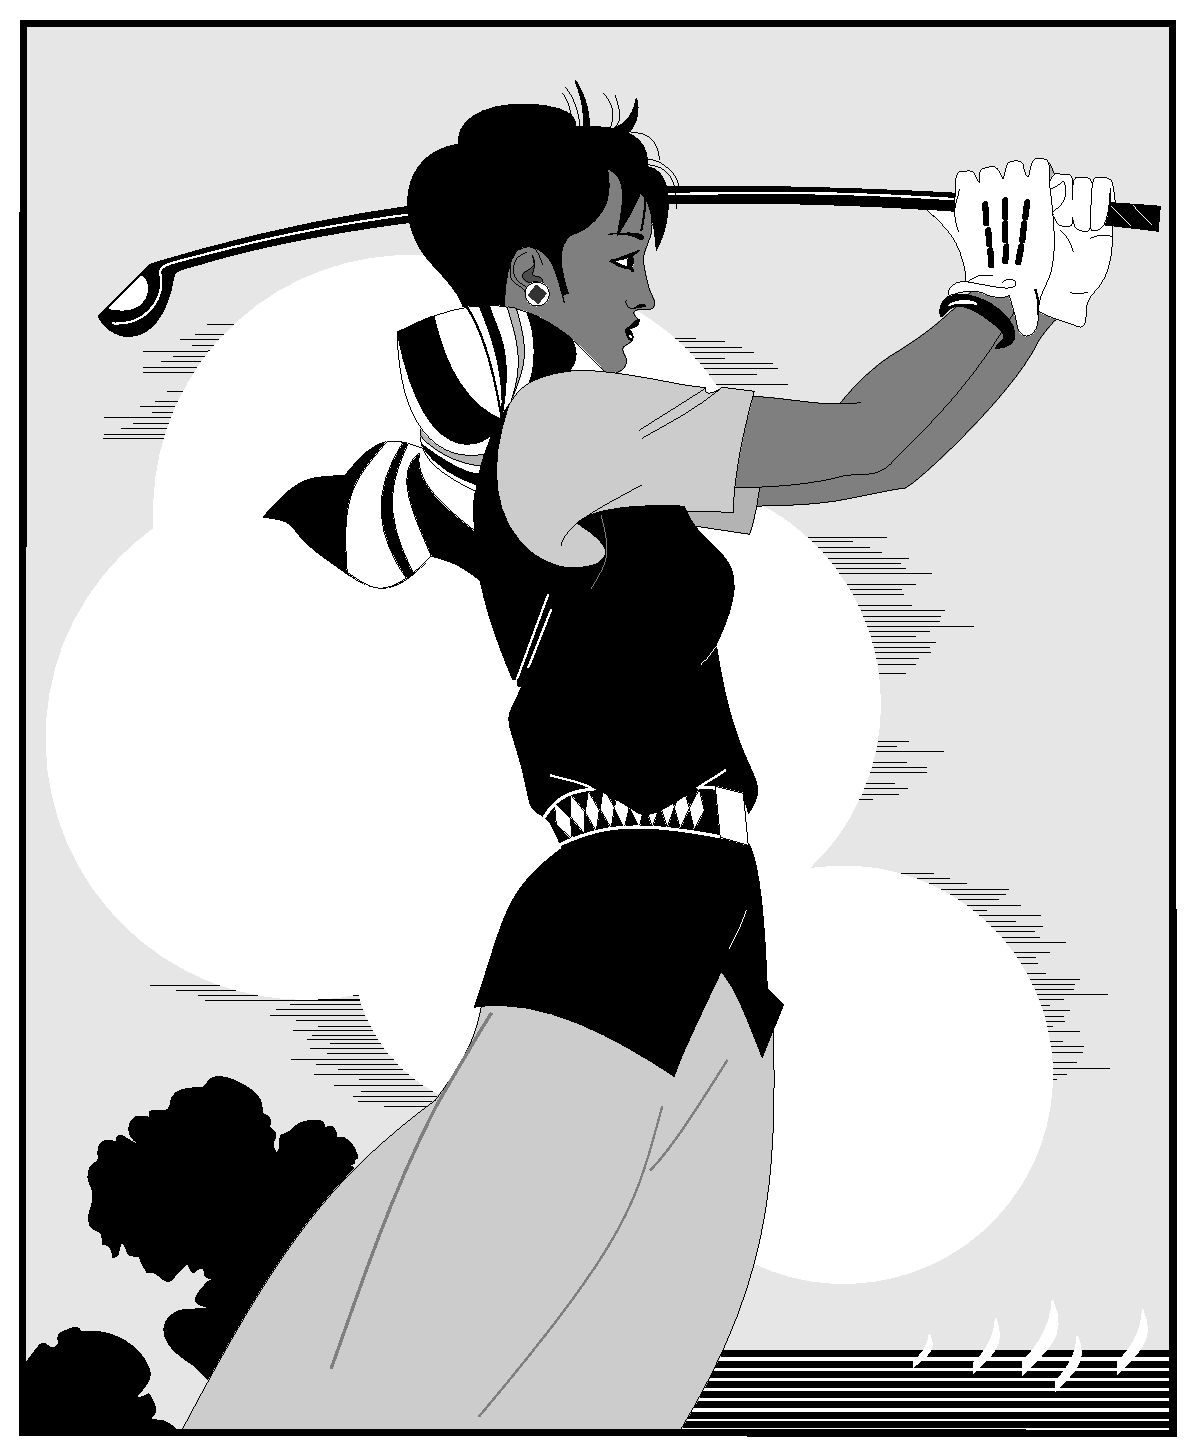
\includegraphics[width = 0.4\textwidth]{golfer}
%\bicaption[golfer5]{}{\xiaosi[0]打高尔夫球的人}{Fig.$\!$}{The person playing golf}\vspace{-1em}
\caption{\xiaosi[0]打高尔夫球的人}
\label{fig:appA}
\end{figure}

附录中\equref{eq:appA}:
\begin{align}
a & = b \times c \\
E & = m c^2
\label{eq:appA}
\end{align}
